\documentclass[11pt]{beamer}
\usepackage[UTF8,scheme=plain]{ctex}
\usepackage{listings}
\usepackage[utf8]{inputenc}
\usepackage[T1]{fontenc}
\usepackage{amsmath}
\usepackage{amsfonts}
\usepackage{amssymb}
\usepackage{graphicx}
\usetheme{Boadilla}

\usepackage{framed} % 可以用 \begin{shaded},即背景色块
\definecolor{shadecolor}{rgb}{0.9,0.9,0.9}

\newcommand{\kong}[1][0.5]{\vspace{#1cm}}

\begin{document}
	\author{ 路毅 \hspace{0.3cm} 曲阜师范大学 }
	\date{\number\year 年 \number\month 月 \number\day 日}
	\title{数学物理方法第四章}

\begin{frame}
	\maketitle
\end{frame}

\kaishu

\begin{frame}{第四章:解析函数的幂级数表示}
\begin{itemize}
	\item 第一节:函数项级数的基本性质
	\vspace{1cm}
	\item 第二节:幂级数与解析函数
	\vspace{1cm}
	\item 第三节:洛朗级数
	\vspace{1cm}
	\item 第四节:单值函数的孤立奇点
\end{itemize}
\end{frame}

\begin{frame}{数项级数}
复数级数:
\begin{equation}
\sum^\infty_{n=0} \omega_n = \omega_0 + \omega_1 + \cdots
\end{equation}
其中$\omega_n = u_n + i v_n$。
\begin{equation}
\sum_{n=0}^{\infty}\omega_n \rightarrow s= \sigma + i \tau
\Leftrightarrow \left\{
\begin{aligned}
& \sum_{n=0}^{\infty} u_n \rightarrow \sigma, \\
& \sum_{n=0}^{\infty} v_n \rightarrow \tau.
\end{aligned}
\right.
\end{equation}

\kong[0.5]
绝对收敛: $\sum_n |\omega_n| $收敛。

\kong[0.5]
条件收敛: $\sum_n \omega_n $收敛,但$\sum_n |\omega_n| $不收敛。
\end{frame}

\begin{frame}{数项级数}
\kong[0.5]
绝对收敛的复数项级数可以重排。

\kong[0.5]
例:两个复数项级数$s=\sum_n \omega_n, s^\prime=\sum_n \omega^\prime_n$绝对收敛,那么它们的乘积为
\begin{equation}
s s^\prime = (\sum^\infty_{k=0} \omega_k) ( \sum^\infty_{l=0} \omega^\prime_l) = \sum^\infty_{n=0} \sum^n_{k=0} \omega_k \omega^\prime_{n-k},
\end{equation}
在上式最后一步,将$(\sum^\infty_{k=0} \omega_k) ( \sum^\infty_{l=0} \omega^\prime_l)$中的各项做了重新组合,不影响整个级数的收敛性,以及收敛值。
\end{frame}

\begin{frame}{函数项级数:一致收敛}
和函数:若$\sum_n f_n (z)$对于定义域$E$上每一点$z$都收敛至$f(z)$,则称$f(z)$是级数$\sum_n f_n (z)$的和函数。

\kong[0.5]
一致收敛:若函数$f(z)$的定义域为$E$,$\forall \epsilon >0$,$\exists N$,当$n>N$时,$\forall z \in E$,有
\begin{equation}
| f(z) - S_n (z) | < \epsilon,
\end{equation}
其中$S_n(z) = \sum^n_{k=0} f_k (z)$。那么我们说$\sum_n f_n(z)$在$E$上{\color{blue}一致收敛}于$f(z)$。

\kong[0.5]
柯西一致收敛准则:$\forall \epsilon >0, \exists N$,当$n>N$时,$\forall z \in E$,有
\begin{equation}
| f_{n+1}(z) + \cdots + f_{n+p}(z) | < \epsilon, p=1,2,3,\cdots
\end{equation}
这是一致收敛的充要条件。
\end{frame}

\begin{frame}{魏尔斯特拉斯M-判别法}
魏尔斯特拉斯M-判别法:若有正数列$M_n, n=0,1,2,\cdots$对任意$z \in E$都有
\begin{equation}
| f_n (z) | \leq M_n, n=0,1,2,\cdots
\end{equation}
且$\sum_n M_n$收敛,则$\sum_n f_n(z)$在$E$上绝对收敛且一致收敛,则$\sum_n M_n$称为$\sum_n f_n(z)$的强级数(或优级数)。

\kong[1]
定理4.1 若$\forall n = 0,1,2,\cdots$ $f_n(z)$在$E$上连续,且$\sum_n f_n(z)$一致收敛于$f(z)$,则
\begin{equation}
f(z) = \sum_{n=0}^{\infty} f_n (z)
\end{equation}
在$E$上连续。
\end{frame}

\begin{frame}{内闭一致收敛}
定理4.2 若$\forall n = 0,1,2,\cdots$,$f_n(z)$在曲线$C$上连续,且在$C$上一致收敛于$f(z)$,则
\begin{equation}
\int_C f(z) dz = \sum_{n=0}^{\infty} \int_C f_n(z) dz,
\end{equation}

\kong[1]
定义4.2 设级数$\sum_{n=0}^{\infty} f_n(z)$的各项均在区域$D$内有定义,若$\sum_{n=0}^{\infty} f_n(z)$在$D$的任一有界闭子区域上一致收敛,则称级数在$D$内“内闭一致收敛”。
\end{frame}

\begin{frame}{魏尔斯特拉斯定理}
定理4.3(魏尔斯特拉斯定理)设级数$\sum_{n=0}^{\infty} f_n (z)$的各项均在区域$D$内解析,且级数在区域$D$内“内闭一致收敛”于$f(z)$,则
\begin{itemize}
	\item [i] $f(z) = \sum_n f_n(z)$在区域$D$内解析
	\item [ii] 在$D$内级数可逐项求导至任意阶,且
	\begin{equation}
	f^{(p)} (z) = \sum_n f^{(p)}_n (z), p=1,2,3,\cdots
	\end{equation}
	\item [iii] $\sum_n f^{(p)}_n (z)$在$D$内内闭一致收敛于$f^{(p)}(z)$。
\end{itemize}
\end{frame}

\begin{frame}{幂级数的收敛性}
阿贝尔定理:如果级数$\sum_n c_n z^n$在$z_0 \neq 0$收敛,则它在以$O$为圆心并通过$z_0$的圆$K: |z|<|z_0|$内绝对收敛,且内闭一致收敛。

\kong[0.5]
证明:
\begin{equation}
\sum_n |c_n z^n| = \sum_n |c_n z^n_0| | z/z_0|^n,
\end{equation}
由于$\sum_n c_n z^n_0$收敛,所以各项的模必有上界,即
\begin{equation}
|c_n z^n_0 | \leq M,
\end{equation}
所以
\begin{equation}
\sum_n |c_n z^n| = \sum_n |c_n z^n_0| | z/z_0|^n
\leq M \sum_n |z/z_0|^n,
\end{equation}
在$K: |z|<|z_0|$内部,$|z/z_0|<1$,所以$\sum_n |c_n z^n|$收敛,即$\sum_n c_n z^n$绝对收敛。
\end{frame}

\begin{frame}{幂级数的收敛性}
在$K$内任意一个闭圆$|z|\leq \rho$($\rho < |z_0|$)上,
\begin{equation}
|c_n z^n| \leq |c_n| \rho^n,
\end{equation}
前面已经证明,$\sum_n |c_n| \rho^n$收敛,所以上式说明$\sum_n c_n z^n$具有强级数,根据魏尔斯特拉斯M-判别法,$\sum_n c_n z^n$在$K$内闭圆上一致收敛。

\kong[0.5]
推论:若$\sum_n c_n z^n$在$z=z_1$点发散,则$\sum_n c_n z^n$在以原点为圆心并通过$z_1$的圆的外部(即$|z|>|z_1|$)必定处处发散。
\end{frame}

\begin{frame}{$\sum^\infty_{n=0} c_n z^n$收敛/发散的分类讨论}
\begin{itemize}
	\item [1] $\forall z \neq 0$,$\sum_{n=0}^{\infty}c_n z^n$发散,例如
	\begin{equation}
	1 + z + 2^2 z^2 + \cdots n^n z^n + \cdots
	\end{equation}
	$\forall z \neq 0$,通项都不收敛,故级数发散。
	\item [2] $\forall z$, $\sum_{n=0}^{\infty} c_n z^n$均收敛,例如
	\begin{equation}
	1 + z + \frac{z^2}{2^2} + \cdots + \frac{z^n}{n^n} + \cdots
	\end{equation}
	$\forall z$,$\exists N$,使得$n>N$时,$|z|/n < 1/2$,所以级数收敛。
	\item [3] $\sum_{n=0}^{\infty} c_n z^n$有不为0的收敛点,也有发散点。
	在这种情况下,根据阿贝尔定理,一定存在一个有限正数$R$,在$|z|=R$内绝对收敛,在$|z|=R$外发散,所以可定义{\color{blue}收敛半径}$R$。
\end{itemize}
\end{frame}

\begin{frame}{收敛半径}
如果$\lim\limits_{n \rightarrow \infty} | c_{n+1} / c_n | = l$,或$\lim\limits_{n \rightarrow \infty} |c_n|^{1/n} = l$,或$\lim\limits_{n \rightarrow \infty}sup |c_n|^{1/n} = l$,
则收敛半径为
\begin{equation}
R = \left\{
\begin{aligned}
&1/l, 	&\text{当$l$为有限值且不为零时}, \\
&0, 	&\text{当$l=\infty$时}, \\
&\infty, &\text{当$l=0$时}
\end{aligned}
\right.
\end{equation}

\kong[1]
例:
\begin{equation}
e^x = 1 + x + \frac{x^2}{2!} + \cdots + \frac{x^n}{n!} + \cdots
\end{equation}
因为$\lim\limits_{n \rightarrow \infty} | \frac{1/(n+1)!}{1/n!}| = 0$,所以收敛半径为$\infty$。
\end{frame}

\begin{frame}{例:几何级数}
几何级数
\begin{equation}
1 + z + z^2 + \cdots + z^n + \cdots
\end{equation}
因为
\begin{equation}
\lim\limits_{n \rightarrow \infty} 1/1 = 1,
\end{equation}
所以收敛半径为 $R=1$,即$ |z|<1$时几何级数收敛,其和函数为$1/(1-z)$,用等比数列前$n$项和取极限即可得到。

\kong[0.5]
问:$\sum_n z^n/n, \sum_n z^n/n^2$的收敛半径分别是多少?
\end{frame}

\begin{frame}{收敛级数的各项系数的意义}
若在区域$D$内任意一处
\begin{equation}
\sum_{n=0}^{\infty} c_n (z-a)^n = f(z),
\end{equation}
根据维尔斯特拉斯定理,在$D$内级数可以逐项求导至任意阶,即
\begin{equation}
c_n = f^{(n)}(z)/n!, n=0,1,2,\cdots
\end{equation}
\end{frame}

\begin{frame}{4.2.2 解析函数的幂级数表示}
定理4.5(泰勒定理)设$f(z)$在区域$D$内解析,$a \in D$,若圆$K:|z-a|<R$包含于$D$内,则$f(z)$在$K$内泰勒级数收敛。
\begin{equation}
f(z) = \sum_{n=0}^{\infty} \frac{f^{(n)}(a)}{n!}(z-a)^n,
\end{equation}
\begin{figure}
	\centering
	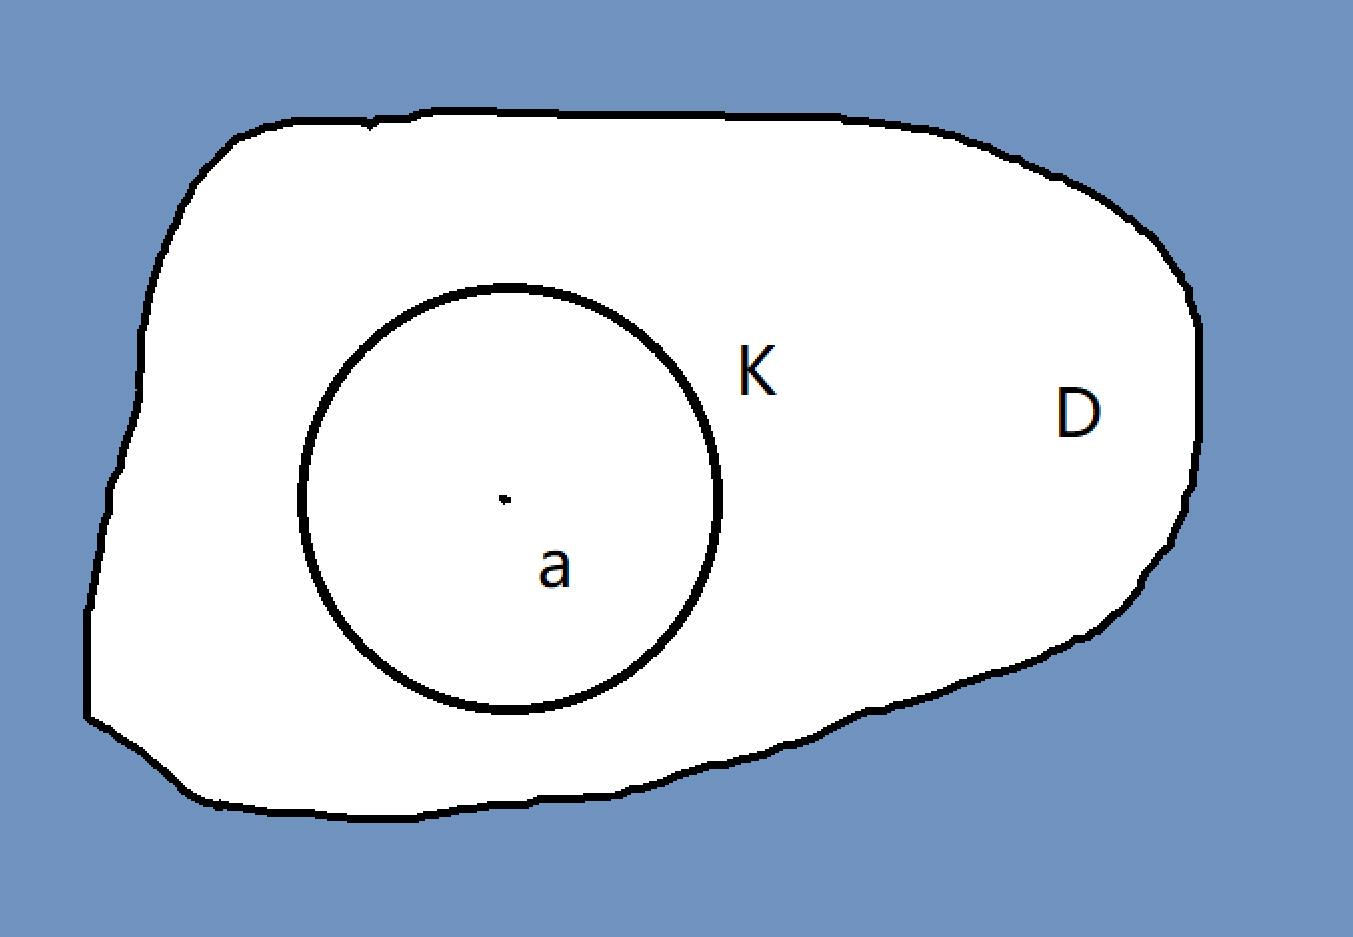
\includegraphics[width=0.5\linewidth]{泰勒定理1}
	\caption{泰勒定理}
	\label{fig:1}
\end{figure}

\end{frame}

\begin{frame}{泰勒定理的证明}
\begin{figure}
	\centering
	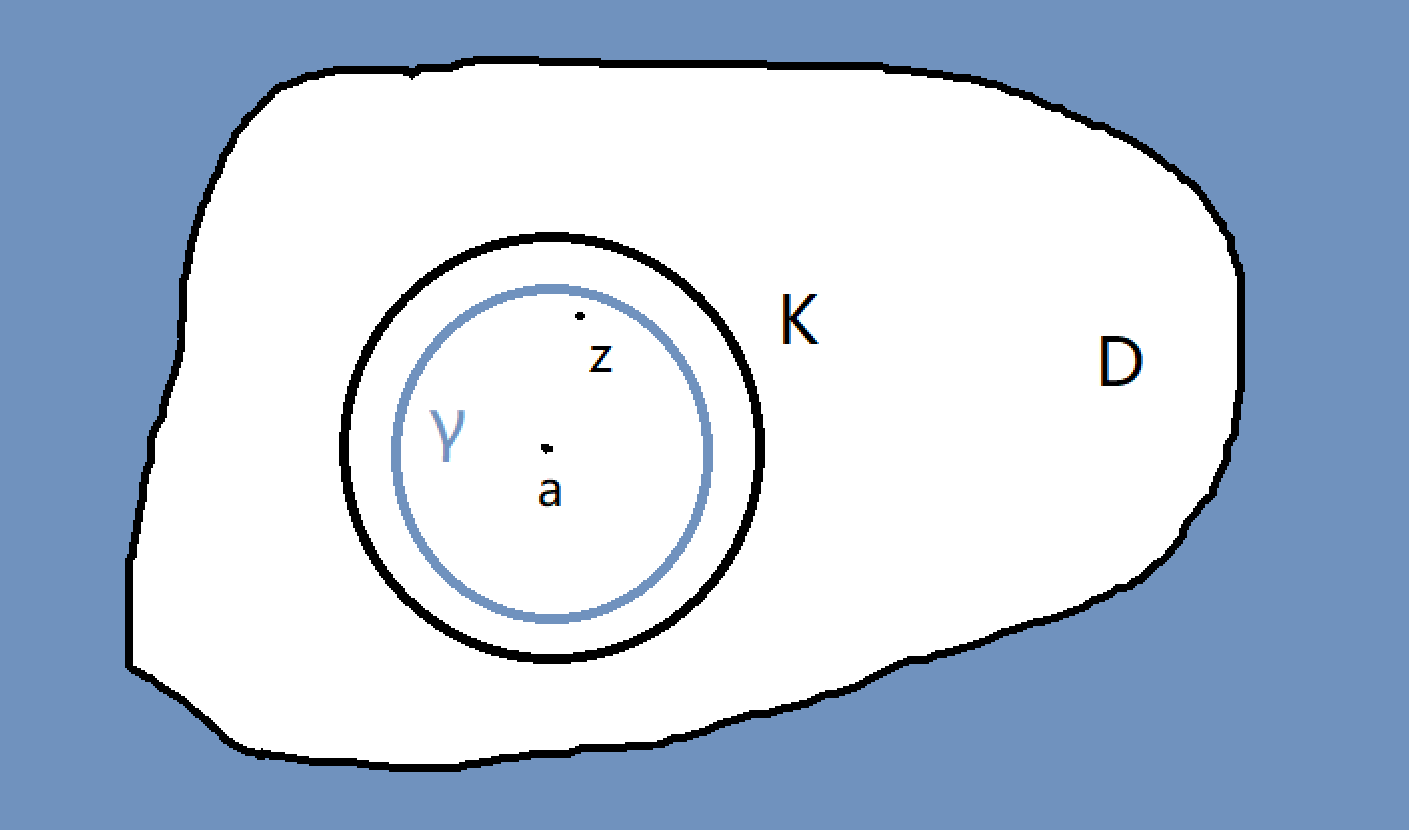
\includegraphics[width=0.5\linewidth]{泰勒定理2}
	\caption{泰勒定理}
	\label{fig:2}
\end{figure}
证明:对$K$内任意一点$z$,都可以作$z$与$K$之间的圆环$\gamma$,其半径$\rho$满足$ |z| < \rho < R$。
根据柯西积分定理
\begin{equation}
f(z) = \frac{1}{2\pi i} \oint_\gamma \frac{ f(\zeta)}{\zeta - z} d \zeta,
\end{equation}

\end{frame}

\begin{frame}{泰勒定理的证明}
进一步,把$f(z)$写作
\begin{equation}
f(z) = \frac{1}{2\pi i} \oint_\gamma \frac{ f(\zeta)}{\zeta - z} d \zeta = \frac{1}{2\pi i} \oint_\gamma \frac{ f(\zeta)}{\zeta - a} \frac{1}{1 - \frac{z-a}{\zeta-a} } d \zeta,
\end{equation}
因为$|\frac{z-a}{\zeta-a}| < 1$,所以$\frac{1}{1 - \frac{z-a}{\zeta-a} } = \sum_{n=0}^{\infty} \frac{(z-a)^n}{(\zeta-a)^n}$,即
\begin{equation}
f(z)= \frac{1}{2\pi i} \oint_\gamma \frac{ f(\zeta)}{\zeta - a} \frac{1}{1 - \frac{z-a}{\zeta-a} } d \zeta
= \sum_{n=0}^{\infty} \frac{(z-a)^n}{2\pi i}  \oint_\gamma \frac{f(\zeta)}{(\zeta-a)^{n+1}} d \zeta,
\end{equation}
利用第三章证明过的结论:$\oint_\gamma \frac{f(\zeta)}{(\zeta-a)^{n+1}} d \zeta = \frac{2\pi i}{n!}f^{(n)}(a)$,得到
\begin{equation}
f(z) = \sum_{n=0}^{\infty} \frac{ f^{(n)}(a) }{ n!} (z-a)^n.
\end{equation}
上述证明过程对$K$内任意一点$z$具有一般性,故泰勒定理得证。
\end{frame}

\begin{frame}{例题}
例2:求$e^z, \cos z, \sin z$在$z=0$的泰勒展开式。

\kong[1]
例3:求多值函数$Ln(1+z)$的各个分支在点$z=0$的泰勒展开,并指出其收敛范围。
$Ln(1+z)$的各支为
\begin{equation}
Ln(1+z) = ln(1+z) + 2k\pi i, k=0, \pm 1, \pm 2, \cdots,
\end{equation}
其中$ln(1+z)$为主值支
\begin{equation}
ln(1+z) = ln|1+z| + i arg(1+z), -\pi < arg(1+z) < \pi.
\end{equation}
在$z=-1$处有奇点,在其他地方都解析,所以根据泰勒定理,收敛半径为1。
\begin{eqnarray}
ln(1+z) &=& \sum_{n=1}^{\infty} \frac{(-1)^{n-1}}{n}z^{n}, \nonumber\\
Ln(1+z) &=& 2k\pi i + \sum_{n=1}^{\infty} \frac{(-1)^{n-1}}{n}z^{n}.
\end{eqnarray}
\end{frame}

\begin{frame}{例题}
函数$\frac{e^z}{1-z}$在$|z|<1$内解析,现求其泰勒展开式。
\end{frame}

\begin{frame}{解析函数的零点}
{\color{blue}$m$阶零点}
若$f(a)=f'(a)=\cdots=f^{(m-1)}(a)=0$,但$f^{(m)}(a) \neq 0$,则称$a$是$f(z)$的$m$阶零点。

\kong[0.5]
{\color{blue}解析函数零点的孤立性}

若$f(z)$是不恒为零的解析函数,$a$是它的一个零点,则必存在$a$的一个邻域,在此邻域内$f(z)$没有其他零点。

证明:因为$f(z)$解析,所以$f(z)$在$a$的邻域内可做泰勒展开
\begin{equation}
f(z) = \sum_{n=0}^{\infty} c_n (z-a)^n,
\end{equation}
由于$f(z)$是不恒为零的解析函数,所以在此邻域内$c_n$不可能全部为零(这个结论是对的,但我们没有给严格证明)。
如果$a$是$m$阶零点,则$f(z) = (z-a)^m \phi(z)$,且$\phi(a) \neq 0$,即$f(z)$的最低阶小量为$(z-a)^m$,它在$a$很小的去心邻域内不可能为零。
\end{frame}

\begin{frame}{双边幂级数:收敛圆环}
如果$(z-a)$,$\frac{1}{z-a}$的两个级数
\begin{eqnarray}
&& c_0 + c_1(z-a) + c_2(z-a)^2 + \cdots \\
&& c_{-1}(z-a)^{-1} + c_{-2} (z-a)^{-2} + \cdots
\end{eqnarray}
分别在$|z-a|<R, |\frac{1}{z-a}|<\frac{1}{r}$收敛,即它们在
\begin{equation}
r < |z-a| < R
\end{equation}
收敛。

\kong[1]
可以定义{\color{blue} 双边级数}:
\begin{equation}
\sum_{n=-\infty}^{\infty} c_n (z-a)^n,
\end{equation}
它在 $r < |z-a| < R$,即一个圆环区域上收敛。
\end{frame}

\begin{frame}{洛朗定理}
洛朗定理:若$f(z)$在圆环区域$H: r< |z-a|<R$解析,则它一定可以展开成{\color{blue}洛朗级数}:
\begin{equation}
f(z) = \sum_{n=-\infty}^{\infty} c_n (z-a)^n,
\end{equation}
其中
\begin{equation}
c_n = \frac{1}{2\pi i} \oint_\gamma \frac{f(\zeta)}{(\zeta-a)^{n+1}} d\zeta, n \in Z
\end{equation}
称为{\color{blue}洛朗系数},其中$\gamma$为满足$r<\rho<R$的同心圆$|z-a|=\rho$。
\end{frame}

\begin{frame}{洛朗定理的证明}
\begin{figure}
	\centering
	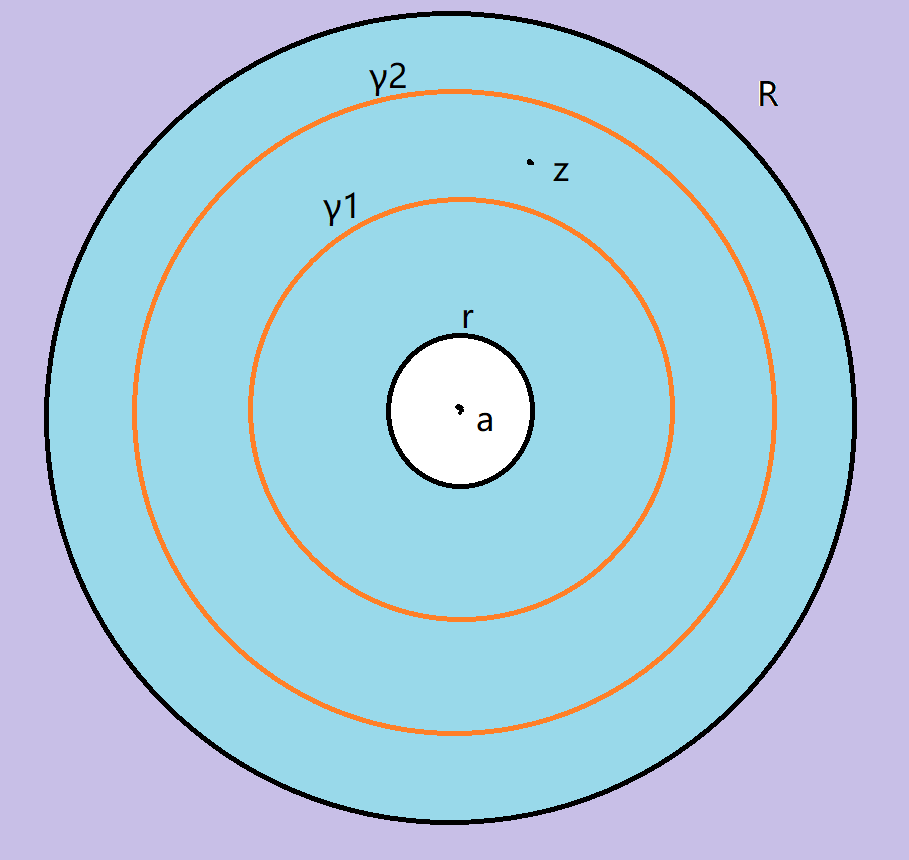
\includegraphics[width=0.4\linewidth]{洛朗定理}
	\caption{洛朗定理的证明}
	\label{fig:}
\end{figure}
对圆环区域内任意一点$z$,作两个辅助圆$\gamma_1, \gamma_2$,其半径$\rho_1, \rho_2$满足
\begin{equation}
r < \rho_1 < |z| < \rho_2 < R,
\end{equation}
\end{frame}

\begin{frame}{洛朗定理的证明}
根据复围线上的柯西积分公式(很容易推广到复围线),
\begin{equation}
f(z) = \frac{1}{2 \pi i} \oint_{\gamma_2 + \gamma^-_1} \frac{f(\zeta)}{\zeta - z} d \zeta
= \frac{1}{2 \pi i} \oint_{\gamma_2} \frac{f(\zeta)}{\zeta - z} d \zeta
-\frac{1}{2 \pi i} \oint_{\gamma_1} \frac{f(\zeta)}{\zeta - z} d \zeta, 
\end{equation}
而
\begin{eqnarray}
\frac{1}{2 \pi i} \oint_{\gamma_2} \frac{f(\zeta)}{\zeta - z} d \zeta 
&=& \frac{1}{2 \pi i} \oint_{\gamma_2} \frac{f(\zeta)}{\zeta - a} \frac{1}{1-(z-a)/(\zeta-a)} d \zeta
\nonumber \\ 
&=& \sum_{n=0}^{\infty}\frac{1}{2 \pi i} \oint_{\gamma_2} \frac{f(\zeta)}{\zeta - a} \frac{(z-a)^n}{(\zeta-a)^n} d \zeta
\nonumber \\
&=& \sum_{n=0}^{\infty} ( \frac{1}{2 \pi i} \oint_{\gamma_2} \frac{f(\zeta)}{(\zeta - a)^{n+1}} d \zeta ) (z-a)^n
\end{eqnarray}
\end{frame}

\begin{frame}{洛朗定理的证明}
在$\gamma_1$上则有
\begin{eqnarray}
\frac{1}{2 \pi i} \oint_{\gamma_1} \frac{f(\zeta)}{\zeta - z} d \zeta 
&=& - \frac{1}{2 \pi i} \oint_{\gamma_1} \frac{f(\zeta)}{z - a} \frac{1}{1-(\zeta-a)/(z-a)} d \zeta
\nonumber \\ 
&=& - \sum_{n=0}^{\infty}\frac{1}{2 \pi i} \oint_{\gamma_1} \frac{f(\zeta)}{z - a} \frac{(\zeta-a)^n}{(z-a)^n} d \zeta
\nonumber \\
&=& - \sum_{n=0}^{\infty} ( \frac{1}{2 \pi i} \oint_{\gamma_1} \frac{f(\zeta)}{(\zeta - a)^{-(n+1) +1}} d \zeta ) (z-a)^{-(n+1)},
\end{eqnarray}
最后一步利用了复围线上的柯西积分定理。
\end{frame}

\begin{frame}{洛朗定理的证明}
将(39-40)带入(38),我们得到
\begin{equation}
f(z) = \sum_{n=-\infty}^{\infty} c_n (z-a)^n,
\end{equation}
其中
\begin{equation}
c_n = \frac{1}{2\pi i} \oint_{\gamma_1} \frac{f(\zeta)}{(\zeta-a)^{n+1}} d\zeta, n \in Z
\end{equation}
$\gamma_1$是半径在$(r,R)$内的任意同心圆,所以洛朗定理得证。

\kong[1]
我们并没有要求$a$点一定是$f(z)$的奇点,所以,洛朗级数也涵盖了泰勒级数,可看作是泰勒级数的推广。
\end{frame}

\begin{frame}{奇点}
孤立奇点:若$f(z)$在$z=a$不解析(无定义或不可导),且存在$z=a$的一个去心邻域,在该邻域内$f(z)$没有其他奇点。反之称作非孤立奇点。

\kong[1]
例子:
\begin{equation}
f(z) = \frac{c}{z-a}; f(z) = \frac{1}{\sin \frac{1}{z}}.
\end{equation}
\end{frame}

\begin{frame}{例题}
例6 函数$f(z) = \frac{1}{(z-1)(z-2)}$分别在$0<|z-1|<1, 0<|z-2|<1$内做洛朗展开。

\kong[0.5]
例7 $f(z) = \frac{\sin z}{z}$在$0<|z|<\infty$做洛朗展开。

\kong[0.5]
例8 $f(z) = e^z + e^{\frac{1}{z}}$在 $0<|z|<\infty$做洛朗展开。

\kong[0.5]
例9 $f(z) = \frac{1}{(z-1)(z-2)}$在$|z|<1, 1<|z|<2, 2<|z|<\infty$做洛朗展开。
\end{frame}

\begin{frame}{单值函数的孤立奇点}
$f(z)$在孤立奇点$z=a$的去心邻域(去心邻域都是圆环)内可做洛朗展开
\begin{equation}
f(z) = \sum_{n=-\infty}^{\infty} c_n (z-a)^n,
\end{equation}
称$\sum_{n=0}^{\infty}c_n (z-a)^n$为在$a$点的正则部分,$\sum_{n=1}^{\infty}c_{-n}(z-a)^{-n}$为在$a$点的主要部分。
\begin{itemize}
	\item [i] 如果主要部分为0,则$z=a$称作可去奇点。
	\item [ii] 如果主要部分为有限多项
	\begin{equation}
	\frac{c_{-1}}{z-a} + \cdots + \frac{c_{-m}}{(z-a)^m}
	\end{equation}
	则$a$为$f(z)$的$m$阶极点。
	\item [iii] 如果主要部分为无限多项,则$a$为本性奇点。
\end{itemize}
\end{frame}

\begin{frame}{可去奇点}
例:$f(z) = \frac{\sin z}{z}$的奇点$z=0$是可去奇点,只需重新定义$f(0)=1$,即可得到一个处处解析的函数。

\kong[1]
可去奇点判定条件(任取其一,三者等价):
\begin{itemize}
	\item [i] $f(z)$在$a$点没有主要成分
	\item [ii] $\lim\limits_{z \rightarrow a} f(z)$存在且有限
	\item [iii] $f(z)$在$a$的充分小邻域内有界。
\end{itemize}

\end{frame}

\begin{frame}{极点}
判定条件(任取其一,三者等价)
\begin{itemize}
	\item [i] $f(z)$在$a$点的主要部分为
		\begin{equation}
	\frac{c_{-1}}{z-a} + \cdots + \frac{c_{-m}}{(z-a)^m}
	\end{equation}
	\item [ii] $f(z)$在$a$的某个去心邻域内能表示成
	\begin{equation}
		f(z) = \frac{\lambda(z)}{(z-a)^m},
	\end{equation}
	其中$\lambda(z)$在$a$的邻域内解析,且$\lambda(a) \neq 0$。
	\item [iii] $g(z) = \frac{1}{f(z)}$以$a$为可去奇点,将$a$作为$g(z)$的解析点看,$a$为$g(z)$的$m$阶零点。
\end{itemize}
\end{frame}

%\begin{frame}{本性奇点}
%$f(z)$的孤立奇点$a$为本性奇点的充要条件是$\lim\limits_{z \rightarrow a} f(z)$不存在,即$z\rightarrow a$时,$f(z)$既不趋于$\infty$(因为它趋于$\infty^\infty$),也不趋于有限值。
%\end{frame}

\begin{frame}{无穷远点}
如果$F(\zeta) = f(1/\zeta)$以$\zeta = 0$为可去奇点、$m$阶极点、本性奇点,则称$f(z)$以$z=\infty$为可去奇点、$m$阶极点、本性奇点。

\kong[0.5]
$f(z)$的正幂部分称为在$z=\infty$的主要部分,
\begin{equation}
c_1 z + c_2 z^2 + \cdots + c_n z^n + \cdots
\end{equation}
余下部分称为正则部分:
\begin{equation}
c_0 + c_{-1}/z + \cdots + c_{-n} / z^n + \cdots
\end{equation}

\end{frame}

\begin{frame}{例子}
例10 $f(z) = \frac{1}{(z-1)(z-2)}$以$z=\infty$为可去奇点,作为解析点来看是二阶零点。

\kong[1]
例11 $m$次多项式$P(z) = a_0 + a_1 z + \cdots + a_m z^m$以$z=\infty$为$m$阶极点。

\kong[1]
例12 $z=\infty$为$f(z)=e^z$的本性奇点。
\end{frame}

\begin{frame}{孤立奇点的判断}
若$f(z)$以$z=a$为孤立奇点,且
\begin{equation}
f(z \rightarrow a)  \rightarrow c_{-m}(z-a)^{-m}, m \in Z
\end{equation}
那么,如果$-m \geq 0$则$a$为$f(z)$的可去奇点;$-m<0$则$a$为$f(z)$的$m$阶极点;$-m \rightarrow - \infty$则$a$为$f(z)$的本性奇点。

\kong[0.5]
证明:在$z=a$的足够小的去心邻域内存在洛朗展开,
\begin{equation}
f(z) = \cdots + \frac{c_{-m}}{(z-a)^m} + \cdots + \frac{c_{-1}}{z-a} + c_0 + c_1(z-a) + \cdots
\end{equation}
如果$z \rightarrow a$时,$f(z) \rightarrow c_{-m}(z-a)^{-m}$,说明$c_{-\infty} = \cdots = c_{-m-1} = 0$。$-m \geq 0$。易得结论。
\end{frame}

\begin{frame}{极点的判断}
例:判断如下函数在$z=0$的奇点类型
\begin{eqnarray}
&& \frac{1+2z+z^2}{z + z^2 + z^3 + \cdots}, \\
&& \cot z = \frac{\cos z}{\sin z } = \frac{1-z^2/2 + \cdots}{z - z^3/6 + \cdots}
\end{eqnarray}
例:判断如下函数在$z=1$的奇点类型
\begin{eqnarray}
&& \frac{1+2z^2}{\ln z} = \frac{1+2z^2}{ \ln(1+(z-1))} = \frac{1+2z^2}{(z-1) - (z-1)^2/2 + \cdots } \\
&& \frac{z-1}{e^{z-1} - e^{1-z}} = \frac{z-1}{2(z-1) + 2(z-1)^3/3! + \cdots }
\end{eqnarray}
\end{frame}

\begin{frame}{极点的判断}

例:判断$\tan (\pi z)$在$z=k+\frac{1}{2}$的奇点类型
\begin{eqnarray}
&& \tan (\pi z) = \frac{\sin (\pi z)}{\cos (\pi z)}
= \frac{ \sin( \pi( k+\frac{1}{2}) + \pi(z - (k+\frac{1}{2})) ) }{\cos( \pi( k+\frac{1}{2}) + \pi(z - (k+\frac{1}{2})) ) }
\nonumber\\
&& = \frac{ \sin( \frac{\pi}{2} + \pi(z - (k+\frac{1}{2})) ) }{\cos( \frac{\pi}{2} + \pi(z - (k+\frac{1}{2})) ) }
\nonumber\\
&& = \frac{1 - \pi^2(z-(k+1/2))^2/2 + \cdots}{- \pi(z-(k+1/2)) + \cdots }
\end{eqnarray}

\end{frame}

\begin{frame}{作业}
课堂选讲:1, 6, 10, 15

\kong[1]
课下练习:3, 4, 9, 12, 13(1-6), 16

\kong[1]
{\color{blue} 有了洛朗级数,留数定理已经呼之欲出,你只需要花二十分钟阅读5.1节,就能晓其大意,快去看看吧!}
\begin{figure}
	\centering
	
\includegraphics[width=0.3\linewidth]{二娃}
	\label{fig:}
\end{figure}


\end{frame}

\end{document}